%! Author = Nhan Huynh
%! Date = 01/12/2021

% Preamble
\documentclass{../tuda-beamer}

% Packages
\usepackage{drawstack}

% Tikz
\tikzstyle{element} = [
node distance = -1pt,
line width = 1pt,
scale = 1.5,
shape = rectangle,
transform shape
]
\tikzstyle{decision} = [
diamond,
draw,
fill = blue!20,
text width = 5em,
text badly centered,
node distance = 3cm,
inner sep = 0pt
]
\tikzstyle{block} = [
rectangle,
draw,
fill = blue!20,
text width = 5.5em,
text centered,
rounded corners,
minimum height = 4em
]
\tikzstyle{line} = [draw, -latex]

% Title information
\authors{Simon Hock}
\authors{Nhan Huynh}
\authors{Daniel Mangold}
\date{01. Dezember 2021}

% Document
\begin{document}

    \maketitle

    \begin{frame}{Überblick}
        \tableofcontents
    \end{frame}


    \section{Statischer vs. dynamischer Typ}
    \begin{frame}{Statischer vs. dynamsicher Typ}
        \begin{itemize}
            \item \textbf{Statischer Typ}:
            \begin{itemize}
                \item Typ, der bei der Variablendeklaration angegeben wird
                \item Ist bei der Kompilierung bekannt
            \end{itemize}
            \item \textbf{Dynamischer Typ}:
            \begin{itemize}
                \item Typ des tatsächlichen Objekts
                \item Ist erst zur Laufzeit bekannt
                \item Kann vom statischen Typ abweichen \(\rightarrow\) Gleich oder Subtyp des statischen
                Typs
            \end{itemize}
            \item Formaler Aufbau
            \begin{center}
                \inlinejava{<Statischer Typ> Bezeichner = <Dynamischer Typ>;}
            \end{center}
        \end{itemize}
    \end{frame}

    \begin{frame}
        \lstinputlisting[style=Java,title=Klasse Rectangle] {codes/Rectangle.java}
    \end{frame}

    \begin{frame}
        \lstinputlisting[style=Java,title=Klasse Square] {codes/Square.java}
    \end{frame}

    \begin{frame}
        \begin{itemize}
            \item Auf welche Methoden können wir mit \inlinejava{rectangle} zugreifen?
            \item Auf welche Methoden können wir mit \inlinejava{square} zugreifen?
            \item Auf welche Methoden können wir mit \inlinejava{rs} zugreifen?
        \end{itemize}

        \br

        \lstinputlisting[
            style=Java,
            title=Vererbung Klasse Rectangle und Square
        ]{codes/Rectangle_and_Square_Example.java}
    \end{frame}

    \begin{frame}[c]
        \begin{note}[title=Information:]
            Ein zentraler Punkt bei Subtypen ist also, dass man beim dynamischen Typ statt der
            eigentlichen Klassen ebenfalls ihre Subtypen verwenden kann. Das gilt für die Deklaration
            von Attributen, Variablen, sowie dem Parameterwert und Rückgabetyp von Methoden.

            \br

            Beim Parameterwert wird deshalb zwischen dem aktualen Wert (der Parameterwert, der
            eingesetzt wird) und dem formalen Wert (der in der Definition des Parameters in der
            Methode steht) unterschieden.
        \end{note}
    \end{frame}

    \begin{frame}
        \begin{figure}[h]
            \centering
            \begin{tikzpicture}[scale=.65, transform shape]
                \begin{scope}[every node/.style={node distance=10pt}]
                    \node (rectangle) at (0, 0) {rectangle};
                    \node (square) at (0, -2.5){square};
                    \node (rs) at (0, -5) {rs};
                \end{scope}
                \begin{scope}[
                    every node/.style={
                    draw,
                    fill=black,
                    line width=1pt,
                    minimum height=30pt,
                    minimum width=15pt,
                    shape=rectangle,
                    }
                ]
                    \node (rectangle-box) at (2.5, 0) {};
                    \node (square-box) at (2.5, -2.5) {};
                    \node (rs-box) at (2.5, -5) {};
                \end{scope}
                \draw[->] (rectangle) -- (rectangle-box);
                \draw[->] (square) -- (square-box);
                \draw[->] (rs) -- (rs-box);
                \begin{scope}[
                    every node/.style={
                    draw,
                    line width=1pt,
                    minimum height=20pt,
                    minimum width=90pt,
                    node distance=-1pt,
                    shape=rectangle,
                    }
                ]
                    \node[fill=black] (rectangle-ref) at (7.5, 1.5) {};
                    \node[below=of {rectangle-ref}] (rectangle-width) {getWidth()};
                    \node[below=of {rectangle-width}] (rectangle-height) {getHeight()};
                    \node[below=of {rectangle-height}] (rectangle-area) {getArea()};
                    \node[below=of {rectangle-area}] (rectangle-circumference) {getCircumference()};

                    \node[fill=black] (square-ref) at (7.5, -3.5) {};
                    \node[below=of {square-ref}] (square-width) {getWidth()};
                    \node[below=of {square-width}] (square-height) {getHeight()};
                    \node[below=of {square-height}] (square-area) {getArea()};
                    \node[below=of {square-area}] (square-circumference) {getCircumference()};
                    \node[below=of {square-circumference}] (square-diagonallength)
                    {getDiagonalLength()};
                \end{scope}
                \draw[->] (rectangle-box.east) -- (rectangle-ref.west);
                \draw[->] (square-box.east) -- (square-ref.west);
                \draw[->] (rs-box.east) -- (square-ref.west);

                \node (width) at (14, -2) {getWidth() in Rectangle};
                \draw[->] (rectangle-width.east) -- (width);
                \draw[->] (square-width.east) -- (width);

                \node (height) at (14, -3) {getHeight() in Rectangle};
                \draw[->] (rectangle-height.east) -- (height.west);
                \draw[->] (square-height.east) -- (height);

                \node (area) at (14, -4) {getArea() in Rectangle};
                \draw[->] (rectangle-area.east) -- (area.west);
                \draw[->] (square-area.east) -- (area);

                \node (circumference-rectangle) at (14, 1) {getCircumference() in Rectangle};
                \draw[->] (rectangle-circumference.east) -- (circumference-rectangle);

                \node (circumference-square) at (14, -6) {getCircumference() in Square};
                \draw[->] (square-circumference.east) -- (circumference-square);

                \node (diagonallength-square) at (14, -7) {getDiagonalLength() in Square};
                \draw[->] (square-diagonallength.east) -- (diagonallength-square);
            \end{tikzpicture}
            \caption{Methodentabelle bezüglich Rectangle und Square Beispiel}
        \end{figure}
    \end{frame}

    \subsection{\texorpdfstring{Statischer Typ \(\neq\) \inlinejava{static}}{Statischer Typ !=
        static}}
    \begin{frame}{Statischer Typ \(\neq\) \inlinejava{static}}
        \begin{itemize}
            \item Statischer Typ: Typ einer Variable, die bei der Variablendeklaration angegeben
            ist.
            \item Schlüsselwort \inlinejava{static}: Klassenattribute/ -methoden (statisch), die
            nicht einzelnen Objekten, sondern deren gesamter Klasse zugeordnet werden.

            \lstinputlisting[
                style=Java,
                title=Schlüsselwort static
            ] {codes/sum_iterative.java}
        \end{itemize}
    \end{frame}

    \subsection{Beispiel - Athene Karte}
    \begin{frame}{Beispiel - Athene Karte}
        \begin{itemize}
            \item Modellierung der Athene Karte
            \item Enthält Namen eines Universitätsmitglied und weitere Information
        \end{itemize}

        \begin{figure}[h]
            \centering
            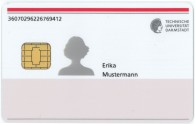
\includegraphics[width=.3\linewidth]{graphics/athena_card_dummy}
            \caption{Quelle: \url{https://www.physik.tu-darmstadt.de/internationales/incoming/general_information_1/athene_card_1/athenecard.en.jsp}}
        \end{figure}
    \end{frame}

    \begin{frame}[c]
        \begin{figure}[h]
            \centering
            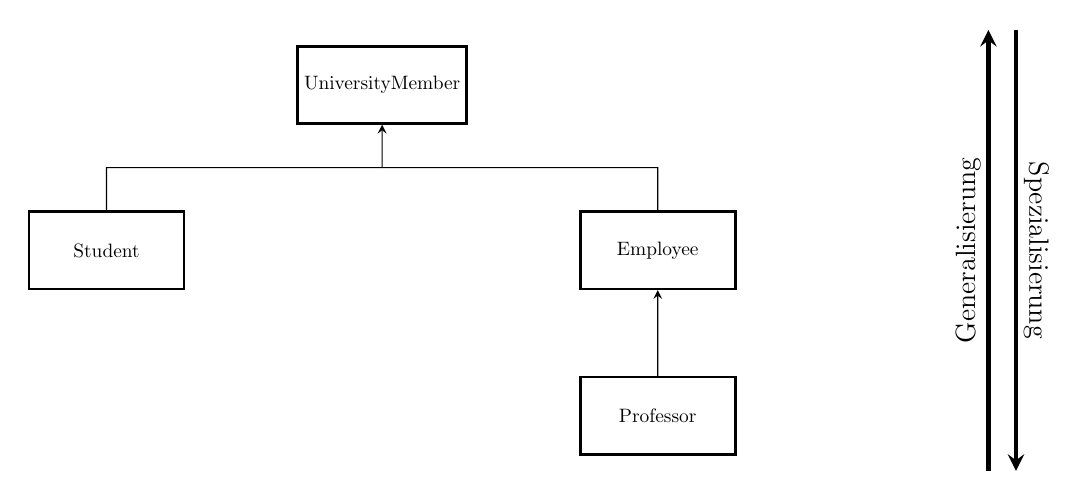
\begin{tikzpicture}[scale=.7, transform shape]
                \begin{scope}[
                    every node/.style={
                    draw,
                    line width=1pt,
                    minimum height=40pt,
                    minimum width=80pt,
                    transform shape,
                    shape=rectangle,
                    }
                ]
                    \node (a) at (0, 0) {UniversityMember};
                    \node (b) at (-5, -3) {Student};
                    \node (c) at (5, -3) {Employee};
                    \node (d) at (5, -6) {Professor};

                    \draw[-stealth] (0, -1.5) -- (a);
                    \draw (b.north) -- (-5, -1.5) -- (0, -1.5);
                    \draw (c.north) -- (5, -1.5) -- (0, -1.5);
                    \draw[-stealth] (d) -- (c);
                \end{scope}

                \draw[-stealth, ultra thick] (11, -7) -- node[rotate=90, above]
                    {\Large Generalisierung} (11, 1);
                \draw[-stealth, ultra thick] (11.5, 1) -- node[rotate=270, above]
                    {\Large Spezialisierung} (11.5, -7);
            \end{tikzpicture}
            \caption{Typhierarchie - Universitätsmitglieder}
        \end{figure}
    \end{frame}
    \begin{frame}[allowframebreaks, c]
        \lstinputlisting[style=Java, title=Klasse UniversityMember]{codes/UniversityMember.java}
    \end{frame}

    \begin{frame}{Dokumentation von nicht implementierten Methoden}
        \begin{itemize}
            \item Spezifiziert die Funktionalität der Methode, welche von Subklassen eingehalten
            werden müssen
            \item Subklassen können den Vertrag spezifizieren
        \end{itemize}

        \lstinputlisting[style=Java]{codes/UniversityMember_getID.java}
    \end{frame}

    \begin{frame}[allowframebreaks, c]
        \lstinputlisting[style=Java, title=Klasse Student]{codes/Student.java}
    \end{frame}

    \begin{frame}[c]
        \lstinputlisting[style=Java]{codes/Student_getID.java}
    \end{frame}

    \begin{frame}[allowframebreaks, c]
        \lstinputlisting[style=Java, title=Enum Department]{codes/Department.java}
    \end{frame}

    \begin{frame}[allowframebreaks, c]
        \lstinputlisting[style=Java, title=Klasse Employee]{codes/Employee.java}
    \end{frame}

    \begin{frame}[allowframebreaks, c]
        \lstinputlisting[style=Java, title=Klasse Professor]{codes/Professor.java}
    \end{frame}

    \begin{frame}[allowframebreaks, c]
        \lstinputlisting[style=Java, title=Klasse AthenaCard]{codes/AthenaCard.java}
    \end{frame}


    \section{Racket HtDPL}
    \begin{frame}{Racket HtDPL}
        \begin{itemize}
            \item Sprachumfang: How to Design a Program Language
            \item Funktionale Sprache
            \item Einschränkung auf wenige Konstrukte und vor allem Rekursion
            \item Atomare Ausdrücke
            \item Syntax: Präfix-Notation
        \end{itemize}

        \begin{table}[h]
            \rowcolors{2}{white}{gray!25}
            \centering
            \begin{tabular}{lc}
                \toprule
                \textbf{Notation} & \textbf{Addition zweier Zahlen}
                \\
                \midrule
                Präfix & \(+ \ x \ y\)
                \\
                Infix & \(\ x + y\)
                \\
                Postfix & \(x \ y \ +\)
                \\
                \bottomrule
            \end{tabular}
            \caption{Überblick von Notationen}
        \end{table}
    \end{frame}

    \begin{frame}{Funktionen in Racket}
        \begin{itemize}
            \item Schlüsselwort: \inlineracket{define}
            \item Formaler Aufbau:
            \begin{center}
                \inlineracket{(define (Bezeichner Argumente*) Körper)}
            \end{center}
            \begin{itemize}
                \item Bezeichner: Name der Funktion
                \item Argumente: Optional, werden mit einem Leerzeichen getrennt
                \item Körper: Atomarer Ausdruck
            \end{itemize}
            \item Immer wenn einer Klammer geöffnet wird, wird ein Funktionsaufruf erwartet!
        \end{itemize}
    \end{frame}

    \begin{frame}{Vergleich Java und Racket}
        \begin{minipage}[t]{.5\linewidth}
            \lstinputlisting[style=Java, title=Methode add]{codes/add.java}
        \end{minipage}
        \hfill
        \begin{minipage}[t]{.475\linewidth}
            \lstinputlisting[style=Racket, title=Funktion add]{codes/add.rkt}
        \end{minipage}
    \end{frame}


    \section{Rekursion}
    \begin{frame}[c]{Rekursion}
        \begin{center}
            \enquote{Eine Rekursion ist eine Funktion, die sich selbst aufruft. Dabei wird versucht
            das Problem auf eine einfachere Variante des \textbf{gleichen} Problems rekursiv zu
            reduzieren, welches dann gelöst wird.}
        \end{center}
    \end{frame}

    \begin{frame}
        \begin{minipage}{.45\linewidth}
            \begin{itemize}
                \item \textbf{Rekursionsanker}: Ab diesem Punkt bricht die Rekursion ab.
                (Abbruchbedingung)
                \item In Zeile 4 ruft die Funktion sich selbst auf.
                \begin{itemize}
                    \item Ohne Rekursionsanker würde die Funktion sich selbst \emph{endlos}
                    aufrufen. (Endlosrekursion)
                \end{itemize}
            \end{itemize}
        \end{minipage}
        \hfill
        \begin{minipage}{.525\linewidth}
            \begin{figure}[!ht]
                \centering
                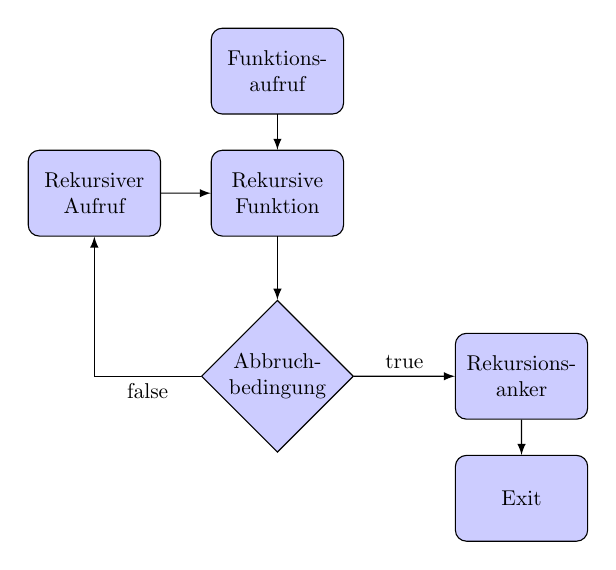
\begin{tikzpicture}[auto, node distance=2cm, scale=0.775, transform shape]
                    \node [block] (function call) {Funktions- \\ aufruf};
                    \node [block, below of = function call] (function recursion)
                    {Rekursive Funktion};
                    \node [decision, below of = function recursion] (decide)
                    {Abbruch- \\ bedingung};
                    \node [block, left of = function recursion, node distance = 3cm]
                    (recursion call) {Rekursiver Aufruf};
                    \node [block, right of = decide, node distance = 4cm]
                    (recursion anchor) {Rekursions- \\ anker};
                    \node [block, below of = recursion anchor, node distance = 2cm] (exit) {Exit};
                    \begin{scope}[every path/.style = {line}]
                        \path (function call) -- (function recursion);
                        \path (function recursion) -- (decide);
                        \path (decide) -| node [near start] {false} (recursion call);
                        \path (recursion call) -- (function recursion);
                        \path (decide) -- node {true} (recursion anchor);
                        \path (recursion anchor) -- (exit);
                    \end{scope}
                \end{tikzpicture}
                \caption{Flow-Chart zu rekursiven Aufruf}
            \end{figure}
        \end{minipage}
    \end{frame}

    \subsection{Vergleich iterativ - rekursiv}
    \begin{frame}{Vergleich iterativ - rekursiv}
        Wir möchten die Gaußsche Summenformel implementieren.

        \begin{equation}
            0 + 1 + 2 + ... + n = \sum_{k = 0}^n = k
        \end{equation}
    \end{frame}

    \begin{frame}{Gaußsche Summenformel - Iterativ}
        \lstinputlisting[style=Java, title=Gaußsche Summenformel]{codes/sum_iterative.java}
    \end{frame}

    \begin{frame}{Gaußsche Summenformel - Rekursiv}
        \lstinputlisting[style=Java, title=Gaußsche Summenformel]{codes/sum_recursive.java}
    \end{frame}

    \begin{frame}{Gaußsche Summenformel - Rekursiv Visualisierung}
        \begin{table}[h]
            \rowcolors{2}{white}{gray!25}
            \centering
            \begin{tabular}{lll}
                \toprule
                \textbf{Rekursionsebene} & \textbf{Aktueller Aufruf} & \textbf{Zwischenstand}
                \\
                \midrule
                0 & \inlinejava{sum(5)} & \inlinejava{sum(4) + 5}
                \\
                1 & \inlinejava{sum(4)} & \inlinejava{sum(3) + 4 + 5}
                \\
                2 & \inlinejava{sum(3)} & \inlinejava{sum(2) + 3 + 4 + 5}
                \\
                3 & \inlinejava{sum(2)} & \inlinejava{sum(1) + 2 + 3 + 4 + 5}
                \\
                4 & \inlinejava{sum(1)} & \inlinejava{sum(0) + 1 + 2 + 3 + 4 + 5}
                \\
                5 & Zurück zum Aufruf von \inlinejava{sum(0)} & \inlinejava{0 + 1 + 2 + 3 + 4 + 5}
                \\
                4 & Zurück zum Aufruf von \inlinejava{sum(1)} & \inlinejava{1 + 2 + 3 + 4 + 5}
                \\
                3 & Zurück zum Aufruf von \inlinejava{sum(2)} & \inlinejava{3 + 3 + 4 + 5}
                \\
                2 & Zurück zum Aufruf von \inlinejava{sum(3)} & \inlinejava{6 + 4 + 5}
                \\
                1 & Zurück zum Aufruf von \inlinejava{sum(4)} & \inlinejava{10 + 5}
                \\
                0 & Zurück zum Aufruf von \inlinejava{sum(5)} & \inlinejava{15}
                \\
                \bottomrule
            \end{tabular}
        \end{table}
    \end{frame}

    \subsection{Exkurs: Stack}
    \begin{frame}{Exkurs: Stack}
        \begin{itemize}
            \item Jede Rekursionsebene benötigt Informationen für die Berechnung
            \item Benötigte Informationen von jeder Rekursionsebene werden im Normalfall in den
            Stack abgelegt.
        \end{itemize}
    \end{frame}

    \begin{frame}[c]
        \begin{figure}[h]
            \centering
            \scalebox{.6}{
                \begin{drawstack}
                    \startframe
                    \cell{Informationen}
                    \cell{Rückkehradresse}
                    \finishframe{0. Rekursionsebene}
                    \startframe
                    \cell{Informationen}
                    \cell{Rückkehradresse}
                    \finishframe{1. Rekursionsebene}
                    \cell{...}
                    \cell{...}
                    \startframe
                    \cell{Informationen}
                    \cell{...}
                    \finishframe{\(n\)-te Rekursionsebene}
                \end{drawstack}
            }
            \caption{Abstrakte Visualisierung eines Stacks von rekursiven Funktionen}
        \end{figure}
    \end{frame}

    \begin{frame}[c]
        \begin{figure}[h]
            \centering
            \scalebox{.55}{
                \begin{drawstack}
                    \startframe
                    \cell{\inlinejava{5}}
                    \cell{\inlinejava{sum(5 - 1)}}
                    \cellround{\inlinejava{sum(4)}}
                    \cell{...}
                    \finishframe{0. Rekursionsebene}
                    \startframe
                    \cell{\((- \ n \ 1)\)}
                    \cell{\inlinejava{sum(4 - 1)}}
                    \cellround{\inlinejava{sum(3)}}
                    \cell{...}
                    \finishframe{1. Rekursionsebene}
                    \cell{...}
                    \cell{...}
                    \startframe
                    \cell{0}
                    \finishframe{5. Rekursionsebene}
                \end{drawstack}
            }
            \caption{Abstrakte Visualisierung des Stacks von rekursiven Aufruf von \inlinejava{sum}}
        \end{figure}
    \end{frame}


    \section{Arbeitsphase}
    \begin{frame}[c]{Arbeitsphase}
        \begin{center}
            \textbf{\LARGE Selbstständiges Arbeiten}
        \end{center}
    \end{frame}
\end{document}
